\documentclass[a4paper,12pt]{article} % Tipo de documento y tamaño de letra.
\usepackage[utf8]{inputenc} % Para que reconozca caracteres especiales como tildes.
\usepackage[spanish]{babel} % Para definir el idioma y el formato de fechas en español.
\usepackage{amsmath, amssymb} % Paquetes para símbolos y ecuaciones avanzadas (Para hacer una ecuación con un recuadro).
\usepackage{ragged2e}
\usepackage{multicol} % Para crear columnas.
\usepackage{slashed} % Para generar números o variables canceladas (Una línea diagonal sobre el número o variable)
\usepackage{graphicx} % Paquete para poner graficas.
\usepackage{float} % Para poder dejar la imagen en un punto fijo del documento.


\title{Actividad Grupal.} 
\author{Liz Ángel Núñez Torres.} 
\date{\today} 

\begin{document}

\maketitle 

\section*{Problema 1} % Comienza la primera sección.

\begin{justify}
    Un hombre está de pie a un metro del borde de un disco giratorio inmenso, de \(50 \; m.\) de radio. El disco gira a \(1 \; rad/s.\) Calcula y explica:
\end{justify}

\begin{enumerate}
    \item Coeficiente de rozamiento mínimo que tiene que haber entre el suelo y los zapatos del hombre para que se mantenga quieto y no salga despedido.
    \item ¿Qué le sucedería al hombre si avanza un metro hacia el centro del disco?
    \item ¿Qué le sucedería al hombre si se aleja medio metro del centro del disco?
\end{enumerate}

\vspace{\baselineskip}

\subsection*{Solución.}

\begin{justify}
    \textbf{Datos:}
\end{justify}

\begin{multicols}{2}
    \(r = 50 \; m.\)
    
\columnbreak
    \(\omega = 1 \; rad/s.\)
    
\end{multicols}

\begin{justify}
    \textbf{(1)} Como el hombre esta a un metro del borde, tendremos que el radio donde esta ubicado es \(\rightarrow r = 49.\)
\end{justify}

\begin{justify}
    El hombre experimenta dos fuerzas, la fuerza centrípeta \(F_c\) que actua al centro del disco, y la fuerza de rozamiento \(F_r\) que contrarrestra su trayectoria tangencial al disco (Primera ley de Newton).
\end{justify}

\newpage


\begin{justify}
    Para que se el sujeto se mantenga en su sitio la fuerza de rozamiento deberá ser mayor o igual a la fuerza centrípeta.
\end{justify}


\begin{center}
    \(F_r \geq  F_c.\)
\end{center}

\vspace{\baselineskip}


\begin{justify}
    Dado que queremos obtener el valor mínimo de rozamiento trabajaremos de la forma:
\end{justify}

\begin{center}
    \(F_r = F_c.\)
\end{center}

\vspace{\baselineskip}

\begin{justify}
    Donde necesitaremos saber la equivalencia de las fuerzas y otros datos:
\end{justify}

\begin{multicols}{4}
    \(F_r = \mu \cdot N. \)

    \columnbreak

    \(F_c = m \cdot a_c.\)

    \columnbreak

    \(N = m \cdot g.\)

    \columnbreak

    \(a_c = \omega^2 \cdot r. \)
\end{multicols}

\vspace{\baselineskip}

\begin{justify}
    Procedemos a buscar entonces nuestro valor mínimo de fricción.
\end{justify}

\(F_r = F_c \hspace{0.5 cm}  \Longrightarrow \hspace{0.5 cm}  \mu \cdot N = m \cdot a_c  \hspace{0.5 cm}  \Longrightarrow \hspace{0.5 cm} \mu \cdot m \cdot g = m \cdot \omega^2 \cdot r \)

\vspace{\baselineskip}

\begin{center}
    \( \mu = \frac{\slashed{m} \cdot \omega^2 \cdot r }{\slashed{m} \cdot g}\hspace{0.5 cm}  \Longrightarrow \hspace{0.5 cm} \mu = \frac{\omega^2 \cdot r}{g}.\)
\end{center}

\vspace{\baselineskip}

\begin{justify}
    Reemplazamos en la ecuación obtenida los datos dados en el problema: 
\end{justify}

\begin{center}
    \(\mu = \frac{1^2 \cdot 49}{9.81} = 4.99.\)
\end{center}

\vspace{\baselineskip}

\begin{justify}
    El valor mínimo de fricción para que el sujeto permanezca en el disco es:
\end{justify}

\begin{center}
    \[
    \boxed{\mu = 4.99.}
    \]
\end{center}

\newpage

\begin{justify}
    \textbf{(2)} Vamos a ver que sucede si el hombre avanza un metro hacia el centro del disco desde el punto en que calculamos anteriormente la fricción \(\mu.\)
\end{justify}

\begin{justify}
    Usaremos la ecuación obtenida anteriormente y reemplazaremos con los nuevos datos.
\end{justify}

\begin{center}
    \[
    \boxed{\mu = \frac{1^2 \cdot 48}{9.81} = 4.89.}
    \]
\end{center}

\begin{justify}
    Cuando el sujeto se desplaza un metro hacia dentro, la fuerza de fricción que se debe efectuar para mantenerlo en el disco es menor.
\end{justify}

\vspace{\baselineskip}

\begin{justify}
    \textbf{(3)} A continuación, analizaremos que le sucedería al sujeto si estando en el centro del disco se aleja medio metro del mismo.
\end{justify}

\begin{justify}
    Para esto, usaremos la ecuación obtenida en el punto \textbf{(1)} además de ajustar el valor del radio \(r = 0.5.\)
\end{justify}

\begin{center}
    \[
    \boxed{\mu = \frac{1^2 \cdot 0.5}{9.81} = 0.0509.}
    \]
\end{center}

\begin{justify}
    Igual que en el punto \textbf{(2)} la fuerza de fricción necesaria para mantener el sujeto en el disco es menor, por esto, podemos argüir que la fuerza de fricción es directamente proporcional al radio de la circunferencia, dado que al diminuir el radio también disminuye la fuerza de fricción.  
\end{justify}

\newpage 

\section*{Problema 2} % Comienza la segunda sección.

\begin{figure}[h!]
    \centering
    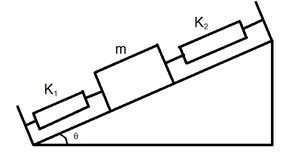
\includegraphics[width=\textwidth]{Imagen actividad G.jpg}
    \caption{El bloque de la figura se encuentra en equilibrio, sujeto por ambos resortes. }
\end{figure}

\begin{justify}
    \textbf{Los datos de cada elemento son los siguientes:}
\end{justify}

\begin{itemize}
    \item Constantes recuperadoras de los muelles: \(K_1 = 70 \; N/m \Longrightarrow K_2 = 50 \; N/m.\)
    \item Masa del cuerpo \(\hspace{0.5 cm} \Longrightarrow \hspace{0.5 cm} m = 10 \; kg.\)
    \item Longitudes originales de los dos muelles \(\hspace{0.5 cm} \Longrightarrow \hspace{0.5 cm} L = 1 \; m.\)
    \item Ángulo de inclinación del plano \(\hspace{0.5 cm} \Longrightarrow \hspace{0.5 cm} \theta = 30. \)
\end{itemize}

\vspace{\baselineskip}

\begin{enumerate}
    \item Con estos datos calcula la posición de equilibrio del bloque, esto es, cuánto se comprime el de abajo, o lo que es lo mismo, que se estire el de arriba.
\end{enumerate}

\subsection*{Solución.}

\begin{justify}
    \textbf{Hacemos el diagrama de cuerpo libre:}
\end{justify}

\begin{figure}[H]
    \centering
    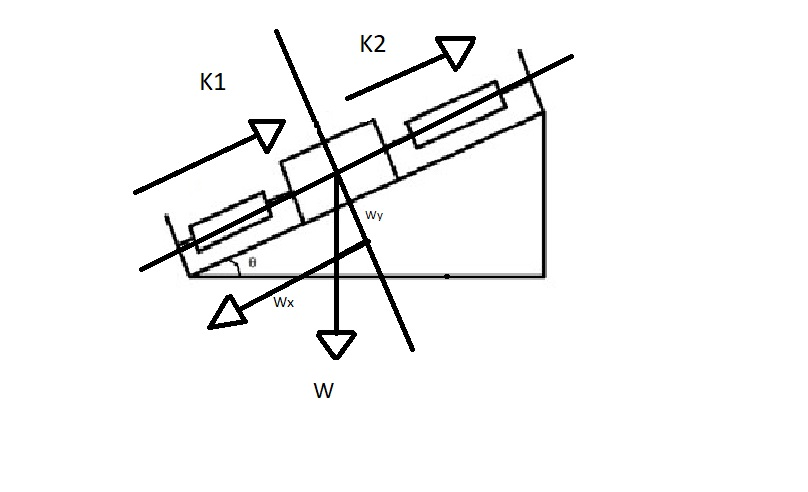
\includegraphics[width=\textwidth]{Diagrama de cuerpo libre.jpg}
    \caption{DLC. }
\end{figure}

\begin{justify}
    El resorte \(K_1\) es comprimido mientras el resorte \(K_2\) ha sido  estirado, por esto en el diagrama de fuerzas ambos vectores tienen la misma dirección y sentido. 
\end{justify}

\begin{itemize}
    \item \(K_1\) emplea una fuerza para recuperar su forma de la compresión que ejerce el bloque. 
    \item \(K_2\) emplea una fuerza para comprimirse del estiramiento que ejerce el bloque. 
    \item El vector \(W_x\) va en dirección y sentido contrario al de los resortes, tal como vemos en el diagrama de cuerpo libre, donde descomponemos \(W\) en sus vectores suma (Hemos exagerado el módulo de \(W_x\) para mostrar el sentido del vector).
\end{itemize}

\newpage

\begin{justify}
    Recordemos que al hablar de resortes debemos aplicar la \textbf{Ley de Hooke} que establece que la fuerza aplicada a un cuerpo es directamente proporcional a su deformación, y se expresa matemáticamente como:
\end{justify}

\begin{center}
    \(F = k \cdot x.\)
\end{center}

\begin{justify}
    Dado que el bloque está en equilibrio, quiere decir que se está aplicando la primera Ley de Newton.
\end{justify}

\begin{center}
    \(\Sigma F = 0.\)
\end{center}

\begin{justify}
    En nuestro caso:
\end{justify}

\begin{center}
    \(K_1 + K_2 - W_x = 0.\)
\end{center}
\begin{justify}
    Vamos a sustituir nuestra variables y proceder con la ecuación.
\end{justify}

\(k_1 \cdot x + k_2 \cdot x - m \cdot g \cdot sin\;\theta  \Longrightarrow x \left(k_1 + k_2\right) = m \cdot g \cdot sin \; \theta .\)

\begin{center}
    \[{x = \frac{ m \cdot g \cdot sin \; \theta }{k_1 + k_2}}.\]
\end{center}

\begin{justify}
    Reemplazamos por los datos:
\end{justify}

\begin{center}
    \[
    \boxed{x =\frac{10 \cdot 9.81 \cdot 0.5}{70+50} = 0.408 \; m. }
    \]
\end{center}

\begin{itemize}
    \item Por lo tanto, podemos afirmar que el resorte \(K_1\) se comprime \( 0.408 \; m.\) y el resorte \(K_2\) se expande \( 0.408 m.\)
\end{itemize}

\newpage

\section*{Problema 3} % Comienza la tercera sección.

\begin{figure}[h!]
    \centering
    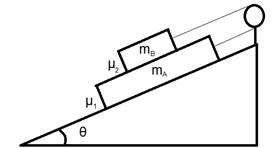
\includegraphics[width=\textwidth]{Imagen2.jpg}
    \caption{Dos bloques de madera se encuentran sobre un plano inclinado, unidos por una polea y una cuerda de masas y efectos despreciables.}
\end{figure}

\begin{justify}
    \textbf{Los datos de cada elemento son:}
\end{justify}

\begin{itemize}
    \item Masas de los bloques \(\hspace{0.5 cm}  \Longrightarrow  \hspace{0.5 cm} m_A = 20 \; kg. \hspace{0.5 cm} m_B = 10.\)
    \item Coeficiente  de rozamiento entre el plano y la masa \(A  \Longrightarrow \hspace{0.5 cm} \mu_1 = 0.2.\)
    \item Coeficiente de rozamiento entre las masas \(A\) y \(B   \Longrightarrow  \hspace{0.5 cm} \mu_2 = 0.3.\)
    \item Ángulo del plano inclinado \(\hspace{0.5 cm} \Longrightarrow \hspace{0.5 cm} 50.\)
\end{itemize}

\begin{justify}
    \textbf{Calcular:}
\end{justify}

\begin{enumerate}
    \item Aceleración y su sentido.
    \item Si el centro del bloque \(B\) está a \(50 \; cm.\) de cada uno de los bloques (dicho de otro modo, que el bloque \(A\) mide \(1 \; m.\)), calcular el tiempo que tarda el centro del bloque \(B\) en llegar al borde.
    \item Valor del ángulo que impediría el movimiento de los bloques. 
\end{enumerate}

\newpage

\section*{Solución}

\begin{justify}
    \textbf{Hacemos el diagrama de cuerpo libre para el bloque \(m_B.\)}
\end{justify}

\begin{figure}[h!]
    \centering
    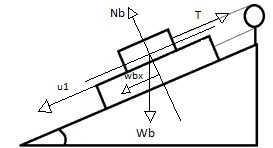
\includegraphics[width=\textwidth]{Bloque b.jpg}
    \caption{DCL}
\end{figure}

\begin{justify}
    Del diagrama de cuerpo libre, aplicamos la segunda ley de Newton para las fuerzas que se efectuan en el plano en el eje de las abcisas.
\end{justify}

\[\Sigma F = m \cdot a.\]

\begin{justify}
    Donde tenemos que:
\end{justify}

\[T - \mu \cdot N_b - W_{bx} = m \cdot a. \]

\[T - 0.3 \cdot \left(10 \cdot 9.81 \cdot \cos (50)\right) - 10 \cdot 9.81 \cdot \sin (50) = 10a.\]

\[T - 18.91 - 75.1 = 10a.\]

\textbf{(1)} \[ T - 94.01 = 10a.\]

\newpage

\begin{justify}
    \textbf{Hacemos el diagrama de cuerpo libre para el bloque \(m_A\)}
\end{justify}

\begin{figure}[h!]
    \centering
    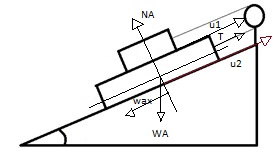
\includegraphics[width=\textwidth]{Bloque a.jpg}
    \caption{DCL}
\end{figure}

\begin{justify}
    Del diagrama de cuerpo libre, aplicamos la segunda ley de Newton para las fuerzas que se efectuan en el plano en el eje de las abcisas.
\end{justify}

\begin{justify}
    Donde tenemos que:
\end{justify}


% \[W_{Ax} - T - \mu_1 - \mu_2 = - m\cdot a\]

%\begin{justify}
 %   Hay que recordar, que la normal \(N_A\) es afectada no solo por el el peso del bloque \(m_A\), si no que también por el peso del bloque \(m_B.\)
%\end{justify}

%\[N_A = \left(m_B + m_A\right) \cdot g \cdot \cos (50) = 189.1\;N\]








\newpage

\begin{justify}
    \textbf{(2)}
\end{justify}






\vspace{\baselineskip}

\hspace{0.5 cm}


\end{document}